\chapter{Ambiente di Simulazione & Attuazione Hardware-in-the-Loop}
\label{cap2}
Una volta consolidato il modello dinamico all'interno dell'ambiente MATLAB/Simulink (descritto nel Capitolo \ref{cap:1}), l'infrastruttura software è stata espansa per supportare l'esecuzione in tempo reale. L'obiettivo di questa fase è trasformare il modello Simulink in un vero e proprio simulatore di volo. Questo simulatore, sviluppato nel presente lavoro di tesi estendendo il modello del Prof. Raktim Bhattacharya\cite{bhattacharya_f16_trim}, hardware e software, visibile nella sua interezza in Figura \ref{fig:global_pil_system}, costituisce lo strumento definitivo per validare le dinamiche di volo, e in un secondo momento, per testare la robustezza delle strategie di controllo automatico (LQR, MPC) che verranno affrontate nei capitoli successivi.

\vspace{0.5cm}

\begin{figure}[H]
	\centering
	% Sostituisci 'sistema_globale_pil.png' con la foto generale del tuo sistema/postazione o dello schema Simulink completo
	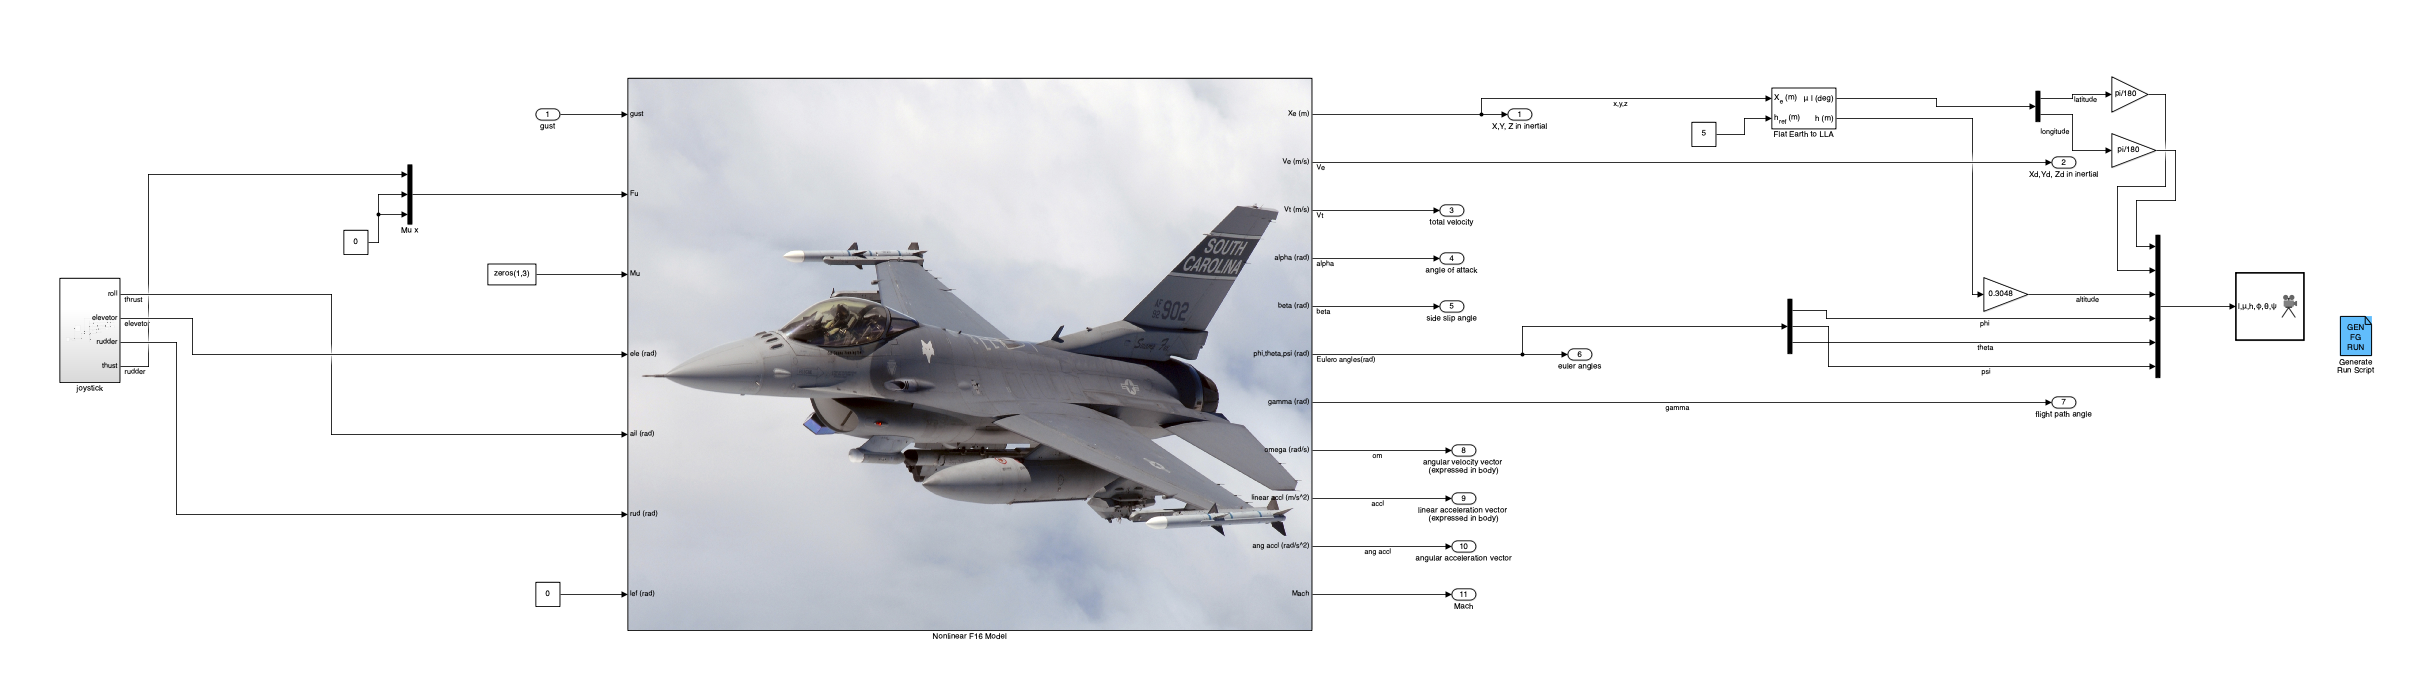
\includegraphics[width=1.1\textwidth, height=150cm, keepaspectratio]{Foto/Simulator.png}
	\caption{Panoramica dell'architettura di simulazione: integrazione tra Simulink e motore di rendering FlightGear.}
	\label{fig:global_pil_system}
\end{figure}



\section{Integrazione con periferiche Thrustmaster HOTAS}
Per interagire fisicamente e in tempo reale con il modello non lineare, il computer che esegue Simulink è stato interfacciato con una periferica di pilotaggio professionale \textbf{Thrustmaster }. L'acquisizione dei comandi avviene tramite appositi blocchi Simulink  strutturati in un \texttt{Sub-System} appositamente implementato per l'acquisizione delle periferiche di gioco (es. \textit{Pilot Joystick} o \textit{Analog Input}). I segnali elettrici analogici provenienti dagli assi vengono acquisiti con un tempo di campionamento rigoroso e sottoposti a condizionamento (normalizzazione, filtraggio del rumore e applicazione di zone morte). 
Nello specifico, la mappatura degli assi permette al pilota di comandare i quattro ingressi primari del velivolo:
\begin{itemize}
	\item \textbf{Manetta (Throttle):} Regola la spinta del propulsore (\texttt{Thrust}).
	\item \textbf{Barra di comando (Stick):} Il movimento longitudinale agisce sull'equilibratore (\texttt{ele}) per il controllo del beccheggio, mentre il movimento laterale comanda gli alettoni (\texttt{ail}) per il rollio.
	\item \textbf{Pedaliera (Pedals):} Comanda il timone di direzione (\texttt{rud}) per l'imbardata.
\end{itemize}
Questi segnali condizionati vengono inviati direttamente agli ingressi del sottosistema aerodinamico e propulsivo, influenzando istantaneamente le derivate di stato del blocco 6-DOF.

\begin{figure}[H]
	\centering
	% Sostituisci 'joystick_subsystem.png' con lo schema Simulink dell'acquisizione Joystick
	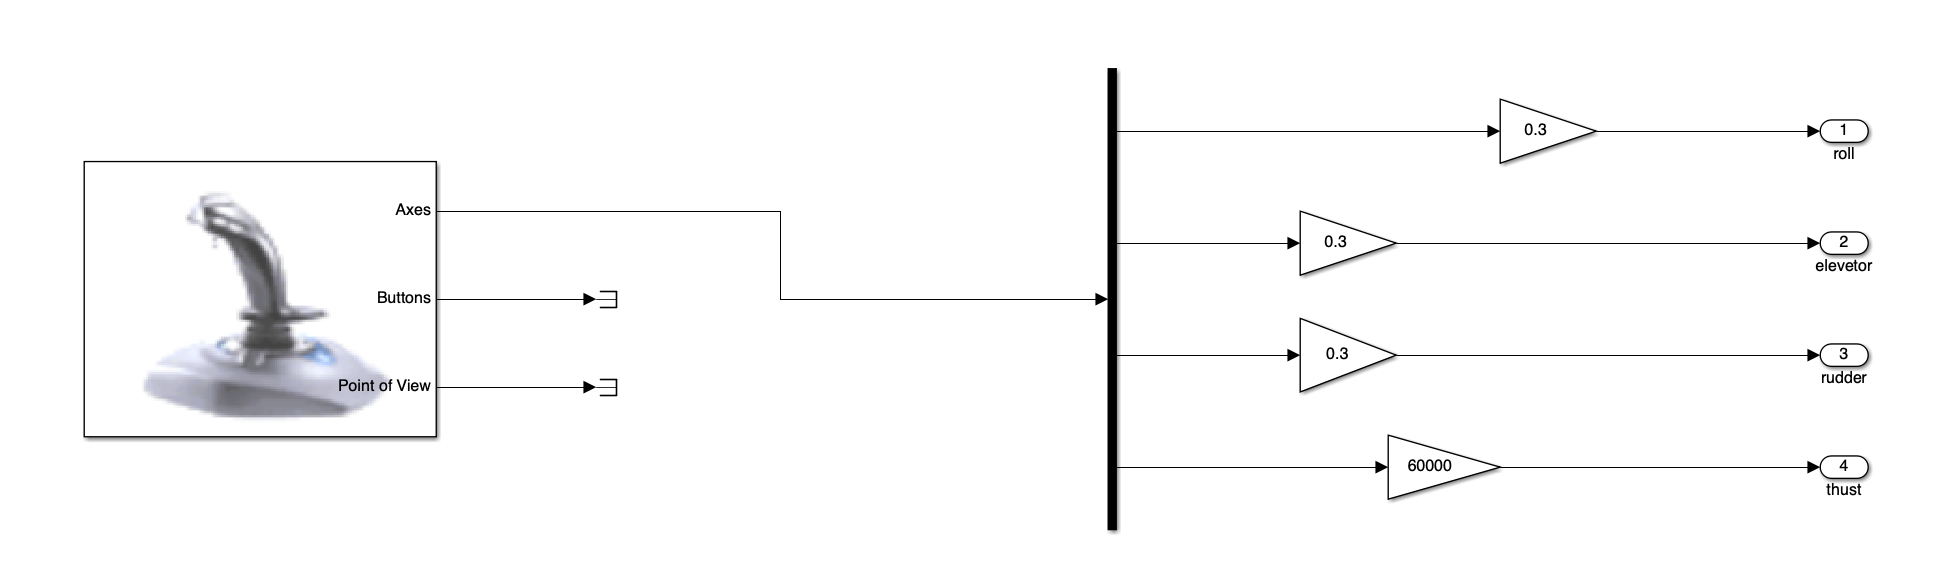
\includegraphics[width=0.85\textwidth, height=6.5cm, keepaspectratio]{Foto/Joystick.png}
	\caption{Sottosistema di acquisizione e condizionamento dei segnali provenienti dal sistema Thrustmaster.}
	\label{fig:hotas_integration}
\end{figure}

\section{Interfacciamento: FlightGear e 
	Aerospace Blockset}
Per fornire un riscontro visivo che sia robusto è importante e di  vitale importanza  registrare le variabili di assetto e delle velocità durante la manovra, per farlo il calcolatore matematico (Simulink) è stato interfacciato con il simulatore di volo open-source \textbf{FlightGear}.
La comunicazione avviene sfruttando i blocchi di rete forniti dall'\textbf{Aerospace Blockset} di MATLAB. Ad ogni istante di campionamento, il vettore di stato globale generato dal blocco 6-DOF viene spacchettato ed inviato a FlightGear tramite protocollo UDP. I dati trasmessi includono:
\begin{itemize}
	\item \textbf{Cinematica Inerziale:} Latitudine, Longitudine e Altitudine.
	\item \textbf{Assetto:} Angoli di Eulero (Rollio $\phi$, Beccheggio $\theta$, Imbardata $\psi$).
\end{itemize}

\subsection{Immagini FlightGear}
In questa sezione vengono riportate le schermate ottenute utilizzando il simulatore FlightGear. Per la simulazione è stata utilizzata la versione 2020.3, integrata con il pacchetto dedicato all'F-16 per permetterne il pilotaggio e il test dei sistemi.

\paragraph{Immagine prima del decollo:}
% Inserisci qui la tua descrizione specifica per la fase a terra
Prima di avviare la simulazione è necessario inizializzare il velivolo sulla pista. Successivamente, tramite l'apposita interfaccia, si attiva la procedura automatizzata che esegue i controlli pre-volo necessari al decollo.

\begin{figure}[H]
	\centering
	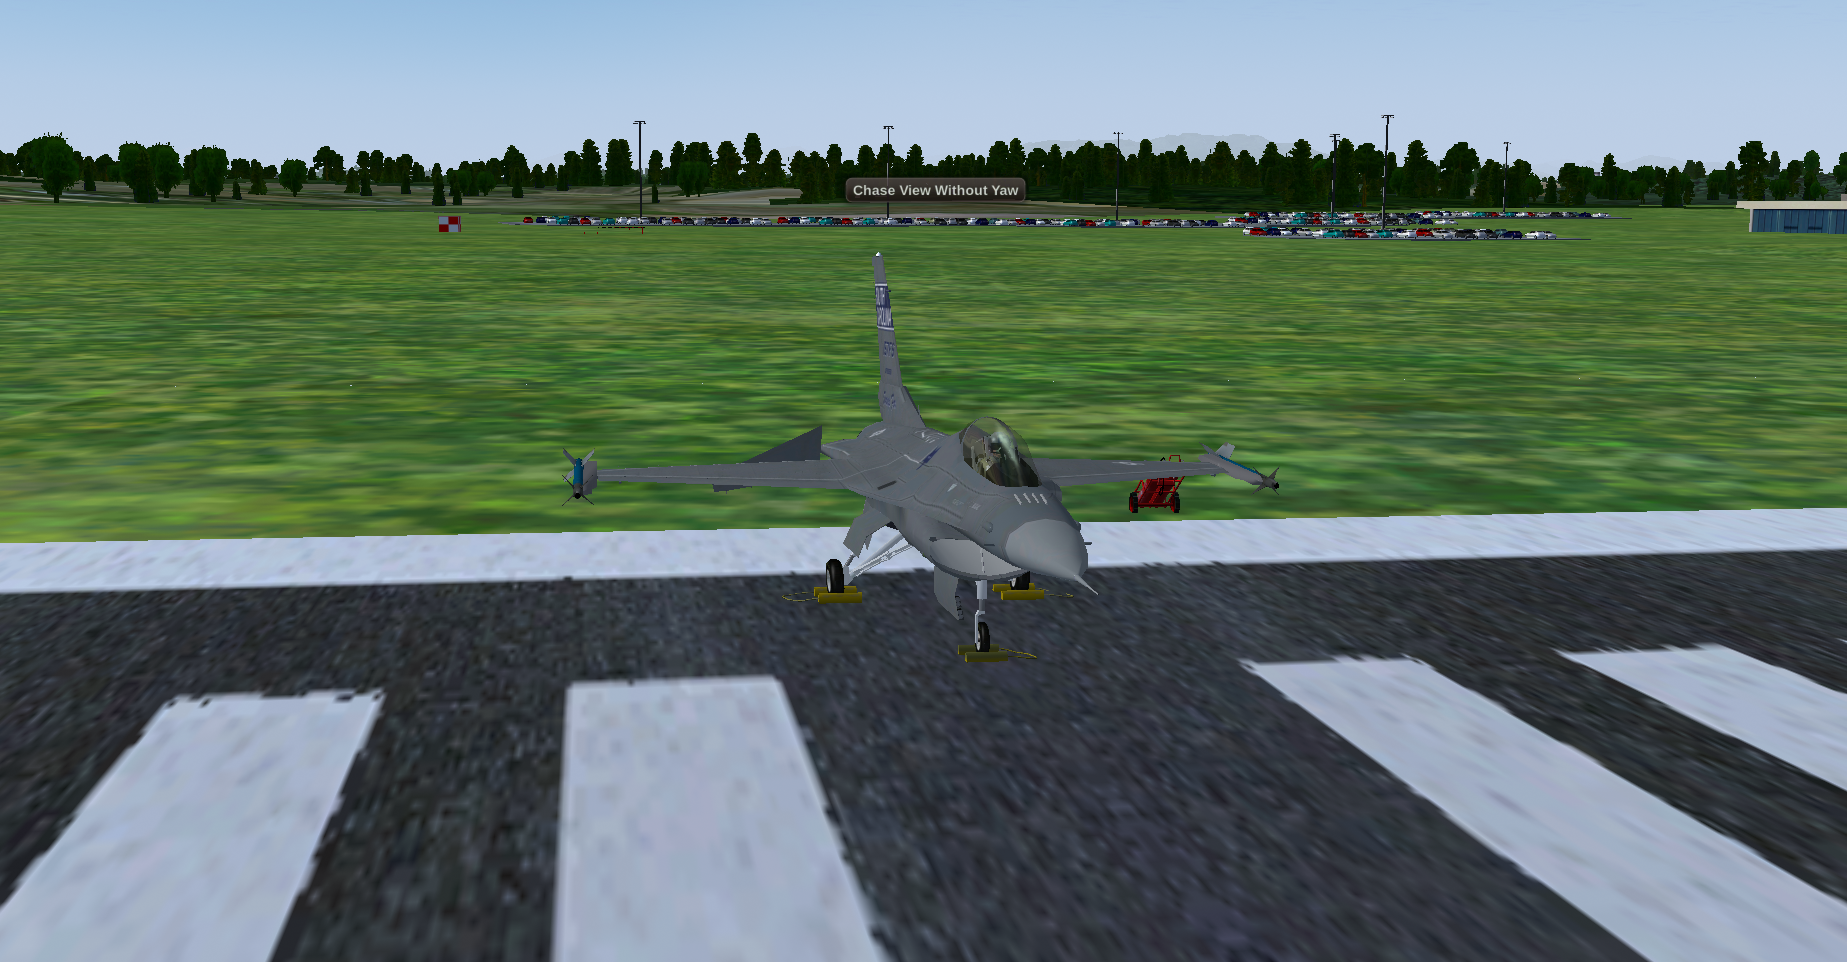
\includegraphics[width=0.85\textwidth, height=6.5cm, keepaspectratio]{Foto/FlightGear/Aterra.png}
	\caption{Visuale a terra dell'aereo prima del decollo.}
	\label{fig:flightGear_terra}
\end{figure}

% --- SECONDA IMMAGINE ---
\paragraph{Volo di crociera}
% Inserisci qui la tua descrizione specifica per il volo di crociera
La Figura \ref{fig:flightGearCrociera} illustra l'aereo in volo di crociera, dimostrando che, anche in assenza di input esterni, il sistema riesce a mantenere il proprio assetto di volo livellato con le tecniche di controllo avazate sviluppate ai capitolo Cap.\ref{cap:lqr} e Cap.\ref{cap:mpc}.
\begin{figure}[H]
	\centering
	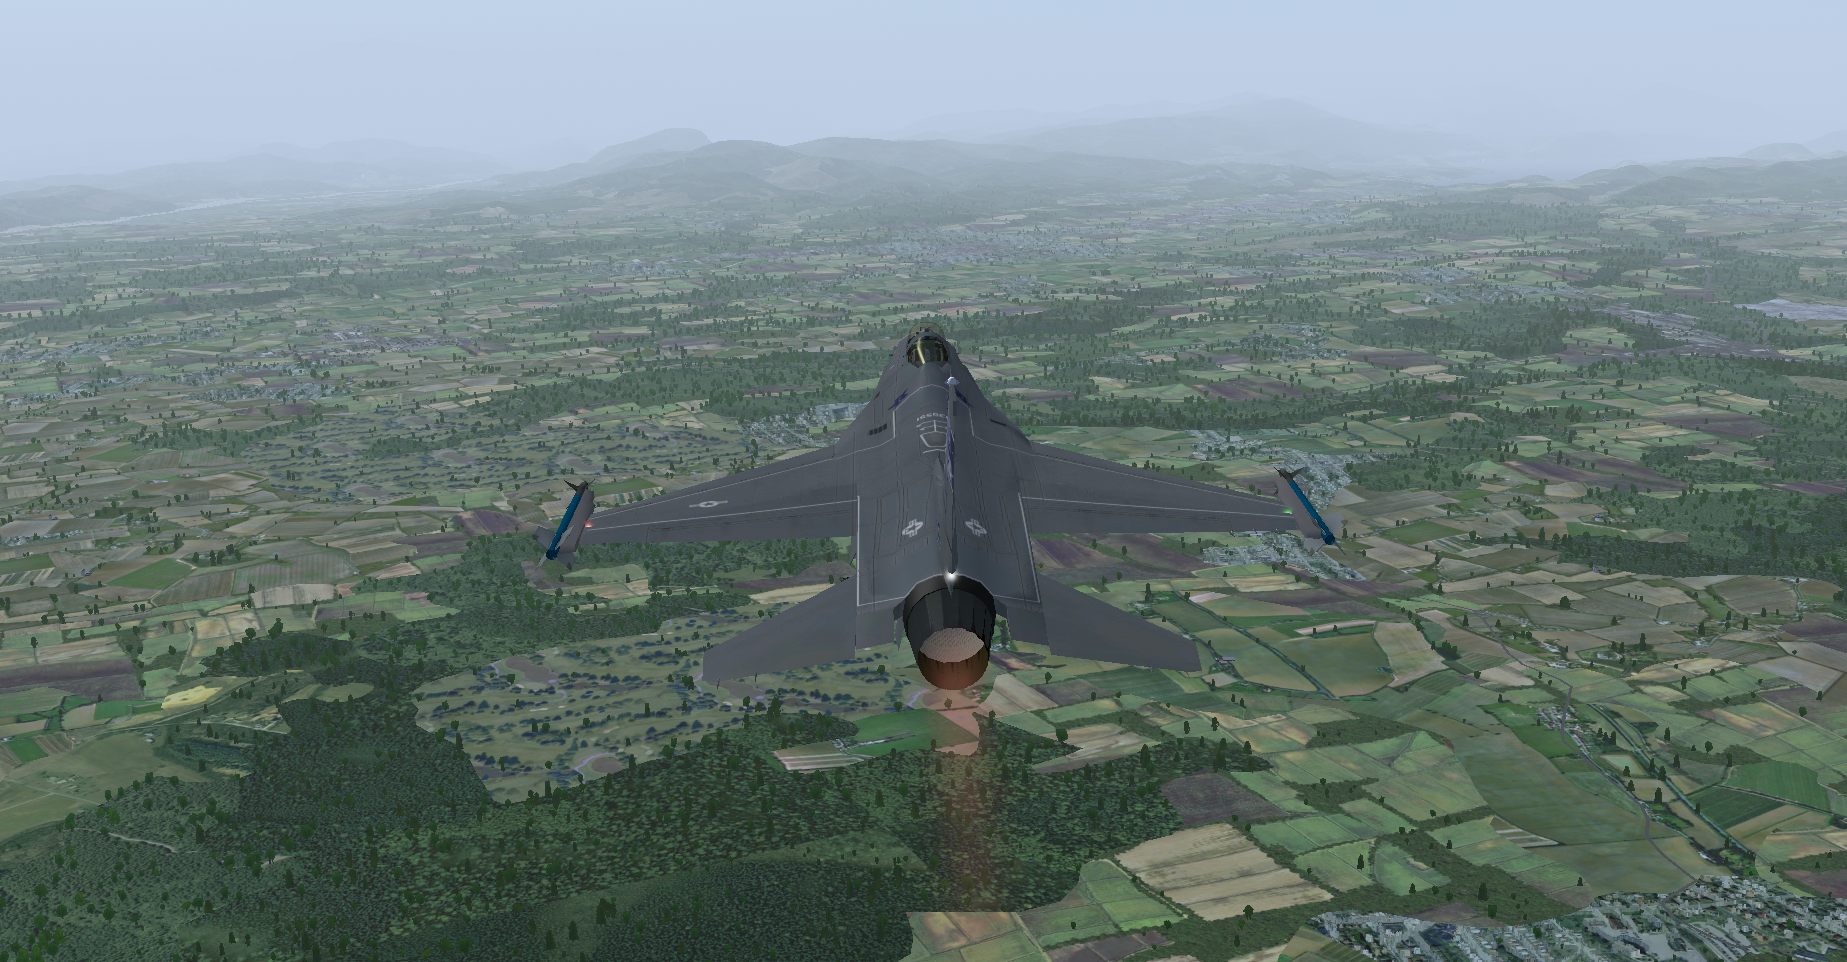
\includegraphics[width=0.85\textwidth, height=6.5cm, keepaspectratio]{Foto/FlightGear/VoloCrociera.png}
	\caption{Visuale FlightGear in volo di crociera.}
	\label{fig:flightGearCrociera}
\end{figure}

% --- TERZA IMMAGINE ---
\paragraph{Visuale interna dell'abitacolo}
% Inserisci qui la tua descrizione specifica per l'abitacolo
Come visibile nella Figura \ref{fig:flightGearAbitacolo}, l'HUD dell'aereo in volo di crociera mostra i valori telemetrici. Tali dati vengono gestiti dal monitor real-time e dal computer di bordo, argomenti trattati diffusamente nel Capitolo \ref{sec:caso_di_studio}.
\begin{figure}[H]
	\centering
	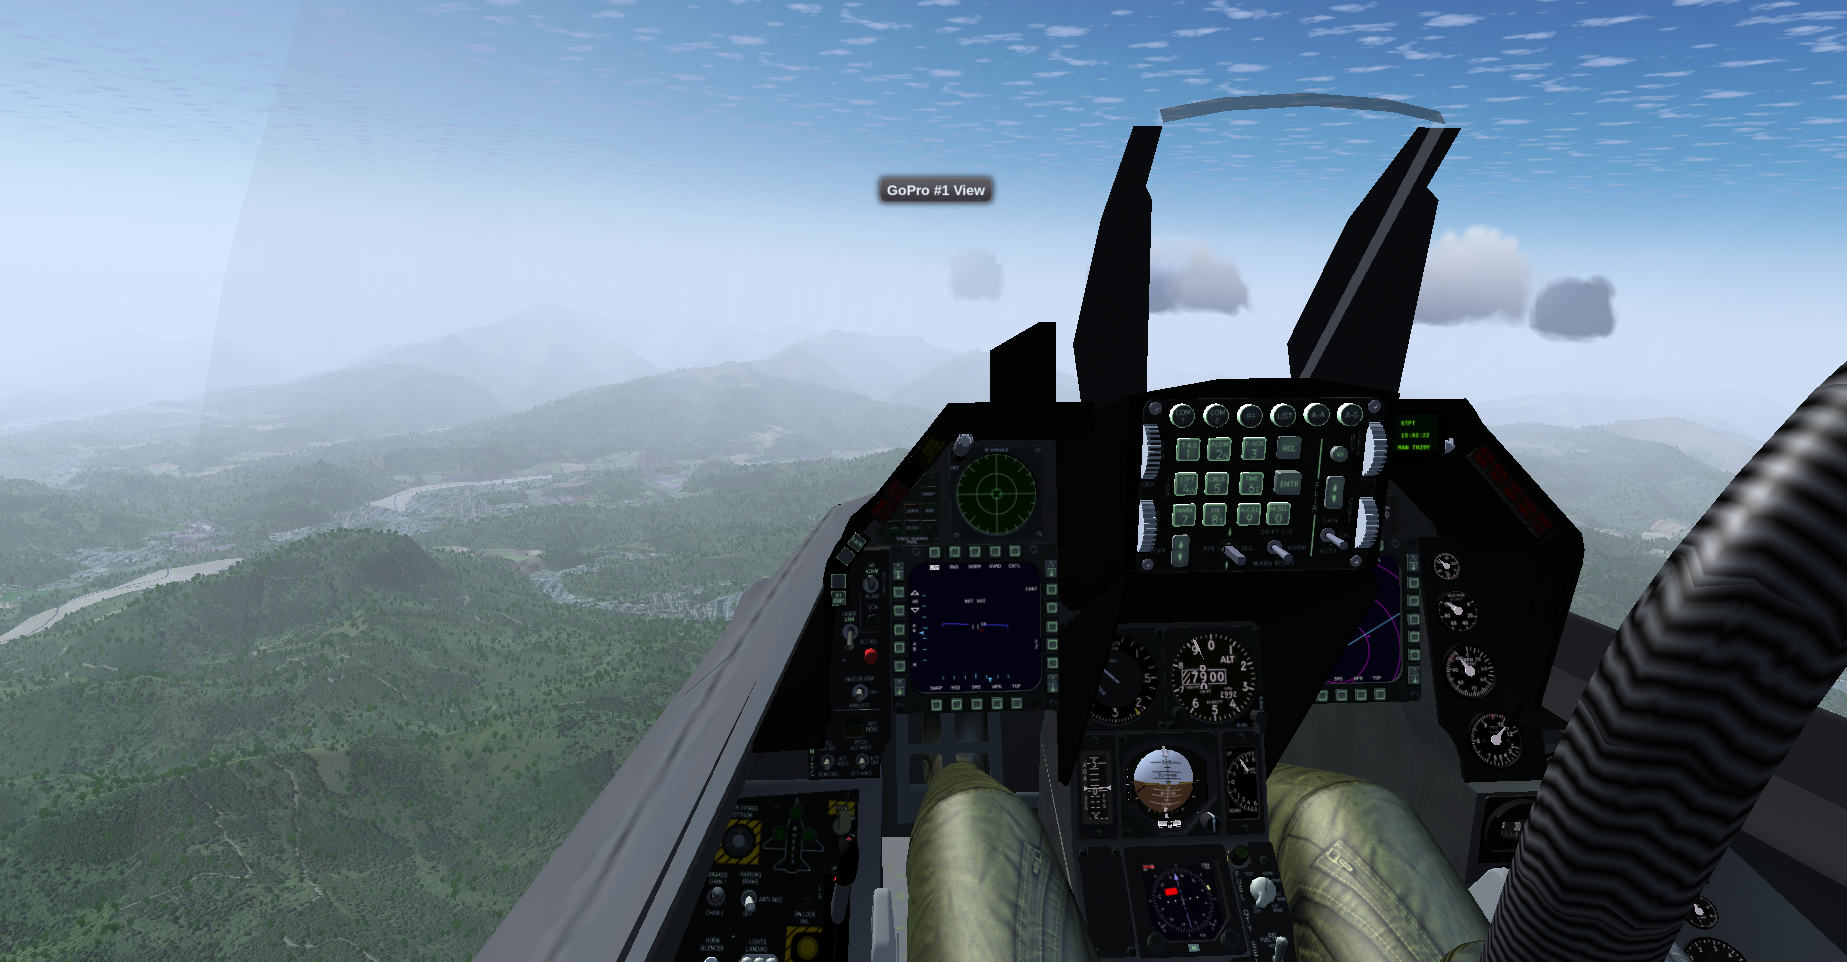
\includegraphics[width=0.85\textwidth, height=6.5cm, keepaspectratio]{Foto/FlightGear/Abitacolo.png}
	\caption{Visuale dell'abitacolo su FlightGear in volo di crociera.}
	\label{fig:flightGearAbitacolo}
\end{figure}

\subsection{Strumenti di Bordo e Telecamere}
\label{sec:cinepresa}
L'impiego di FlightGear non si limita al mero rendering del terreno esterno. Trasmettendo i parametri fisici corretti, FlightGear è in grado di animare in tempo reale il \textit{cockpit} virtuale dell'F-16. Questo permette al pilota di leggere direttamente dall'\textit{Head-Up Display} (HUD) e dagli strumenti analogici valori critici come il numero di Mach, l'altitudine barometrica e l'angolo di rampa ($\gamma$). Inoltre, il sistema permette l'utilizzo delle \textbf{telecamere virtuali (cineprese)} integrate in FlightGear. Il pilota o l'ingegnere di sistema possono variare liberamente il punto di vista durante la simulazione (es. visuale dall'abitacolo, \textit{chase camera} posteriore, visuale \textit{fly-by}) per analizzare visivamente fenomeni dinamici complessi, quali il \textit{Dutch Roll} \cite{etkin_dynamics} o le oscillazioni indotte dai comandi (PIO - \textit{Pilot Induced Oscillations}), che risulterebbero difficili da interpretare unicamente attraverso i grafici temporali.

\begin{figure}
	\centering

	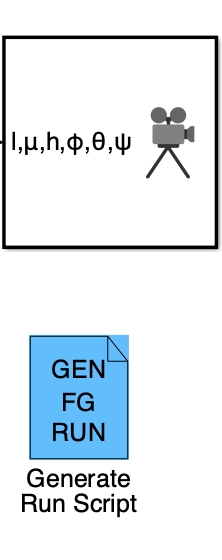
\includegraphics[width=0.30\textwidth, height=7.5cm, keepaspectratio]{Foto/FlightGear.png}
	\caption{Interfacciamento con FlightGear tramite Aerospace Blockset e visualizzazione dell'assetto tramite telecamere esterne e strumentazione di bordo.}
	\label{fig:flightgear_interface}
\end{figure}


% ==========================================
% CAPITOLO 8: EQUILIBRIO E LINEARIZZAZIONE
% ==========================================
\part{Automazione del controllo longitudinale}
